\documentclass[dvipdfmx]{jsarticle} %TikZを使う場合はdvipdfmx忘れずに
\usepackage{ascmac,amsmath,amssymb,amsthm,bm,arydshln,mathcomp,tikz}
\usetikzlibrary{patterns}
\newtheorem{question}{問題}
\newtheorem*{answer*}{解答}
\begin{document}

\begin{question}
  $y = x^3-3x^2+3x-1$ の極値を求めよ.
\end{question}

\begin{question}
  方程式$\sqrt{x} + x = 2$ を解け.
\end{question}

\begin{question}
  $\displaystyle \int_{99}^{100} (x-99)(x-100)$ dx を解け.
\end{question}

\begin{question}
  等式 $0.\dot{9} = 1$ は成り立つか.
\end{question}

\begin{question}
  $0\tcdegree \le x < 360\tcdegree$において, $\displaystyle \frac{d}{dx} \sin x = \cos x$ は成り立つか.
\end{question}

\begin{question}
  点$(x, y)$ が原点を中心とする半径$1$ の円の内部を動くとき, \ 点$(x+y, xy)$ の動く範囲を図示せよ. \ \ \ (1954, 東京大)
\end{question}

\begin{question}
  $x \ge 0$ を定義域とする関数$f(x) = x + \dfrac{1}{x+2}$ の最小値を求めよ.
\end{question}

\begin{question}
以下の漸化式で表される数列$\{a_n\}$ の一般項を求めよ.
$$
a_1=2, \ a_{n+1}=\frac{a_n^2+2}{2 a_n}
$$
\end{question}

\begin{question}
  以下は成り立つか.
\end{question}
  (1) $\emptyset \in \emptyset$ \ \ \ \ 
  (2) $\{\emptyset\} \subset \{\{\emptyset\}\}$

\begin{question}
  解析平均値レポート
\end{question}

\begin{question}
  任意の数列$\{a_n\}, \{b_n\}$ において, $\displaystyle \lim_{n \to \infty} (a_n + b_n) = \lim_{n \to \infty} a_n + \lim_{n \to \infty} b_n$ は成り立つか.
\end{question}

\begin{question}
  $\displaystyle \lim_{n \to \infty} \int_0^n \frac{x^2+1}{x^4+1} dx$ を求めよ.(onenoteに答えあり)
\end{question}

\begin{question}
 方程式$|x-4| = 3x$を解け. 
\end{question}

\vspace{10zw}

\begin{answer*}
\end{answer*}

2. 

\bigskip

$\begin{aligned}
  \sqrt{x} = 2 - x 
  &\Longleftrightarrow (x = (2-x)^2) \land (x \geq 0) \land (2-x \geq 0) \ (必要性と十分性の両方の確認を!)\\
  &\Longleftrightarrow (x^2 -5x + 4 = 0) \land (0 \leq x \leq 2) \\
  &\Longleftrightarrow x = 1
\end{aligned}$

\bigskip

3.

（解答１）
$$
\begin{aligned}
  \displaystyle \int_{99}^{100} (x-99)(x-100) dx
  &= \displaystyle \int_{99}^{100} (x-100+1)(x-100) dx \\
  &= \displaystyle \int_{99}^{100} \{(x-100)^2 + (x-100) \} dx \\
  &= \left[\frac{1}{3} (x-100)^3 + \frac{1}{2} (x-100)^2 \right]_{99}^{100} \\
  &= \frac{1}{3} - \frac{1}{2} \\
  &= -\frac{1}{6}
\end{aligned}
$$

（解答２）
平行移動させて, \ 
$$
\begin{aligned}
  \displaystyle \int_{99}^{100} (x-99)(x-100) dx
  &= \displaystyle \int_0^1 (x-0)(x-1) dx \\
  &= \displaystyle \int_0^1 (x^2 - x) dx \\
  &= \left[\frac{1}{3} x^3 - \frac{1}{2} x^2 \right]_0^1 \\
  &= \frac{1}{3} - \frac{1}{2} \\
  &= -\frac{1}{6}
\end{aligned}
$$

\bigskip

4.

\bigskip

$0.\dot{9} = 0.9 + 0.09 + 0.009 + \dotsb 
= \displaystyle \sum_{n=1}^{\infty} \dfrac{9}{10^n}
= \dfrac{\frac{9}{10}}{1-\frac{1}{10}}
= 1$

\bigskip

6.

$\displaystyle \frac{1}{3} = 1 \div 3  = 0.\dot{3}$ であるから, \ 両辺を$3$ 倍すると, \  %physicsパッケージを入れていると\divが∇・になるため注意

$\begin{aligned}
  3 \times \displaystyle \frac{1}{3}
  &= 3 \times 0.\dot{3} \\
  &= 3 \ (0.3 + 0.03 + 0.003 + \dotsb) \\
  &= 3 \displaystyle \sum_{n=1}^\infty 3 \cdot \frac{1}{10^n} \\
  &= \displaystyle \sum_{n=1}^\infty 9 \cdot \frac{1}{10^n} \ \ \ (極限の性質, \ もっと言うと\varepsilon - N 論法より) \\
  &= 0.\dot{9} \hspace{5zw} (0.\dot{3} \times 3 = 0.\dot{9} はそれほど明らかではない)
\end{aligned}$

したがって, \ $0.\dot{9} = 1$.

\bigskip

座標平面上の点 $(X,Y)$ が求めるべき範囲にある条件は，
\begin{align}
  &x^2 + y^2 < 1 \quad \cdots (1) \\
  &X = x + y \quad \cdots (2) \\
  &Y = xy \quad \cdots (3)
\end{align}
を満たす実数 $x,y$ の組が存在することである。

(2) と (3) をともに満たす $x,y$ は，$t$ の二次方程式
\begin{align}
  t^2 - Xt + Y = 0 \quad \cdots (4)
\end{align}
の2解であるから，(2)(3)を満たす実数 $x,y$ の組が存在する条件は，(4) が実数解を持つことであり，それは判別式を考えて
\begin{align}
  (-X)^2 - 4Y \geq 0 \quad \cdots (5)
\end{align}
と言い換えられる。さらに，その $x,y$ が (1)，すなわち $(x+y)^2 - 2xy < 1$ を満たすのは，
\begin{align}
  X^2 - 2Y < 1 \quad \cdots (6)
\end{align}
のときである。したがって，点 $(X,Y)$ が求める領域に属する条件は (5) かつ (6) が成立することであるから，答えは下図の斜線部である。ただし，境界のうち放物線
\[
  Y = \frac{X^2 - 1}{2}
\]
上の点はすべて含まず，残りの点は含む。

\bigskip

\newpage

\begin{center}
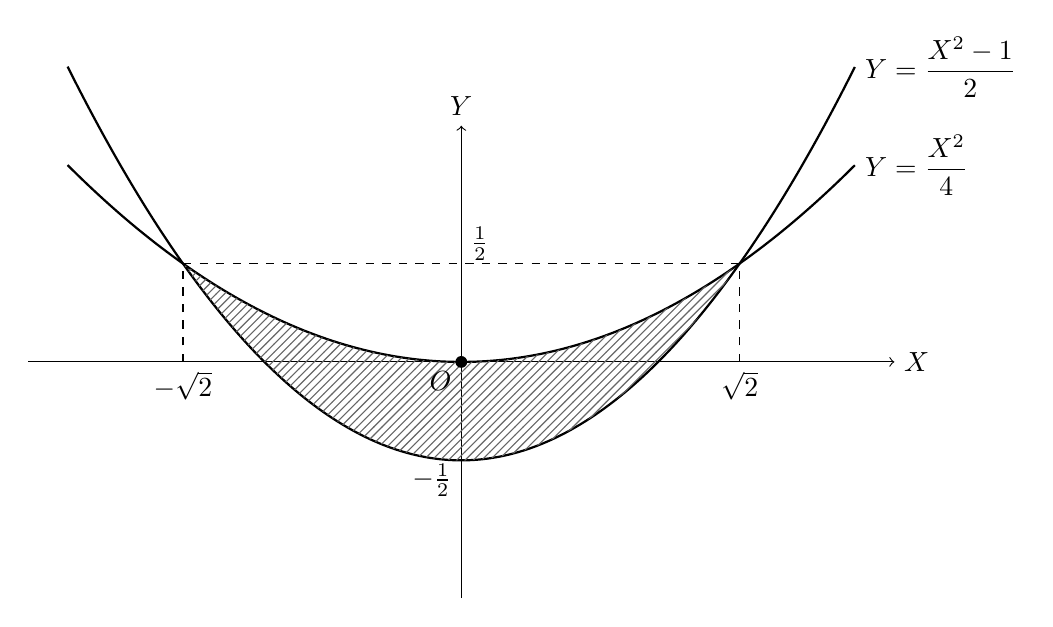
\begin{tikzpicture}[scale=2.5]
  % 軸
  \draw[->] (-2.2,0) -- (2.2,0) node[right] {$X$};
  \draw[->] (0,-1.2) -- (0,1.2) node[above] {$Y$};
  
  % 放物線 Y = X^2/4
  \draw[thick,domain=-2:2,samples=200] 
    plot(\x,{\x*\x/4}) node[right] {$Y=\dfrac{X^2}{4}$};
    
  % 放物線 Y = (X^2 - 1)/2
  \draw[thick,domain=-2:2,samples=200] 
    plot(\x,{(\x*\x-1)/2}) node[right] {$Y=\dfrac{X^2-1}{2}$};
    
  % 斜線部分（-√2 <= x <= √2 の範囲）
  \begin{scope}
    \clip (-1.414,-1.2) rectangle (1.414,1.2); % √2 ≈ 1.414
    \fill[pattern=north east lines,pattern color=black!60]
      plot[domain=-1.414:1.414,samples=200] (\x,{\x*\x/4}) --
      plot[domain=1.414:-1.414,samples=200] (\x,{(\x*\x-1)/2}) -- cycle;
  \end{scope}

  % 点O
  \fill (0,0) circle (0.03) node[below left] {$O$};
  
  % 軸の目盛り
  \draw (0,0.6) node[right] {$\frac{1}{2}$};
  \draw (1.414,0) node[below] {$\sqrt{2}$};
  \draw (-1.414,0) node[below] {$-\sqrt{2}$};
  \draw (0,-0.6) node[left] {$-\tfrac{1}{2}$};

  % 点線
  \draw[dashed] (-1.414,0) -- (-1.414,0.5);
  \draw[dashed] (1.414,0) -- (1.414,0.5);
  \draw[dashed] (-1.414,0.5) -- (1.414,0.5);
\end{tikzpicture}
\end{center}


7.

$$
\begin{aligned}
& c_{m+1}=\frac{a_n^2+2 \sqrt{2} a_n+2}{2 a_n}-\sqrt{2} \Leftrightarrow a_{n+1}+\sqrt{2}=\frac{\left(a_n+\sqrt{2}\right)^2}{2 a_n} \ \  ───\textcircled{\scriptsize 1} \\
& c_{m+1}=\frac{a_n^2-2 \sqrt{2} a_n+2}{2 a_n}+\sqrt{2} \Leftrightarrow a_{n+1}-\sqrt{2}=\frac{\left(a_n-\sqrt{2}\right)^2}{2 a_n} \ \ ───\textcircled{\scriptsize 2}
\end{aligned}
$$
$$
\frac{\textcircled{\scriptsize 1}}{\textcircled{\scriptsize 2}} より, \quad \frac{a_{n+1}+\sqrt{2}}{a_{n+1}-\sqrt{2}}
=\left(\frac{a_{n}+\sqrt{2}}{a_{n}-\sqrt{2}}\right)^2 \\
$$
$b_n=\dfrac{a_{n}+\sqrt{2}}{a_n-\sqrt{2}}$ とおくと, $b_{n+1}=b_n^2$, \quad $b_1=\dfrac{2+\sqrt{2}}{2-\sqrt{2}}=(\sqrt{2}+1)^2$.

ここで, \ 明らかに $a_n>0$ であるから, \ \textcircled{\scriptsize 2} より帰納的に $a_n-\sqrt{2}>0$.

よって, \ $b_n > 0$ ゆえ, \ 両辺$2$を底とする対数をとって,
$$
\begin{aligned}
& \log _2 b_{n+1} =2 \log _2 b_n \\
& \therefore \log _2 b_n 
= 2^{n-1} \log _2(\sqrt{2}+1)^2=\log _2(\sqrt{2}+1)^{2^n} \\
& \therefore b_n=(\sqrt{2}+1)^{2^n}
\end{aligned}
$$
$$
\begin{aligned}
& a_n=\frac{\sqrt{2} b_n}{b_n-\sqrt{2}} ゆえ, \quad a_n=\sqrt{2} \cdot \frac{b_n+1}{b_n-1} \\
& \therefore a_n=\sqrt{2} \cdot \frac{(\sqrt{2}+1)^{2^n}+1}{(\sqrt{2}+1)^{2^n}-1}
\end{aligned}
$$



\end{document}
